

\section{Compiling NVIDIA Jetson Linux with PPS}
\begin{figure}[H]
    \centering
    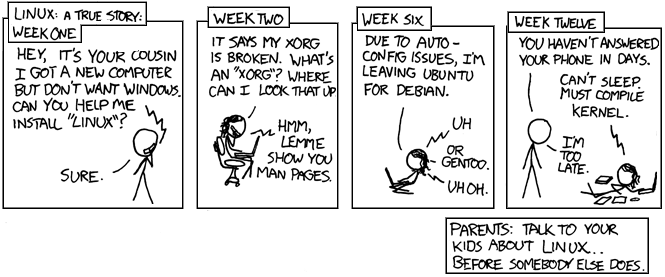
\includegraphics[width=\textwidth]{figures/cautionary.png}
    \caption{Cautionary by XKCD \cite{xkcdCautionary}}
    \label{fig:xkcd_cautionary}
\end{figure}
\subsection{Background}
\gls{pps} is a high precision signal that repeats every seconds provided by a device, typically a GPS receiver, that is used to adjust the system clock time with high accuracy \cite{giomettiLinuxPPSWikiLinuxPPS2007}.
The \gls{pps} signal is often used in combination with \gls{ntpd} to synchronize the system clock with to \gls{utc} with sub millisecond accuracy \cite{giomettiLinuxPPSWikiLinuxPPS2007}.
As \gls{pps} interrupts are hardware based it appears necessary to configure the Linux Kernel as it is responsible for handling interrupts \cite{giomettiLinuxPPSWikiLinuxPPS2007}.
The kernel is the core software component of an operating system that manages system resources and provides a bridge between software applications and hardware devices as visuzlized in Figure \ref{fig:kernel_visualization} \cite{thekerneldevelopmentcommunityInterruptsLinuxKernel}.


The \jx runs an operating system called \gls{jetlinux} which is built on the Linux Kernel \cite{JetsonLinux352023}.
A \gls{pps} signal from one of the \glsps{f9p} is used to sunchronize the clock on the \sr to \gls{utc}, which again is used to synchronize of the cameras using \gls{ptp} \cite{martensPortableSensorRig2022}.

\begin{figure}[H]
    \centering
    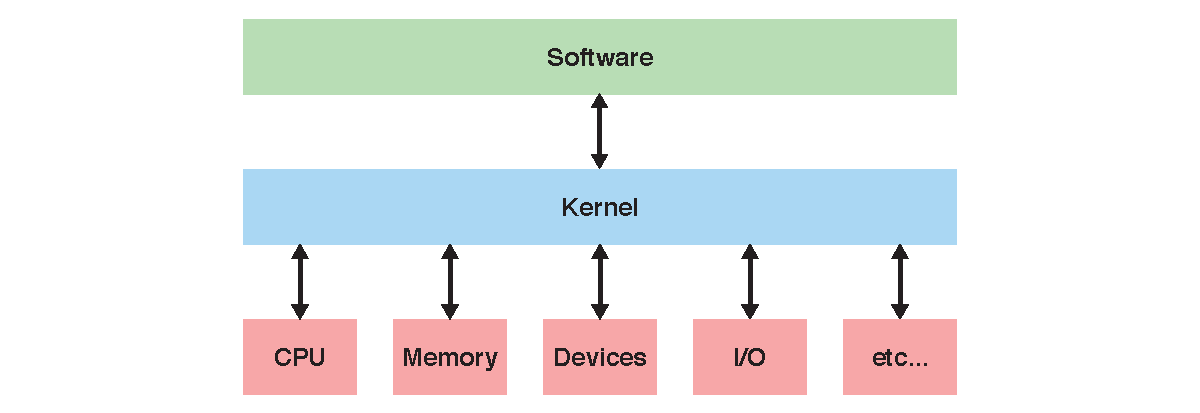
\includegraphics[width=\textwidth]{figures/kernel.pdf}
    \caption{An oversimplification of who the kernel interacts with the hardware and software}
    \label{fig:kernel_visualization}
\end{figure}

\subsection{Results from the \preproject}
During the \preproject \gls{pps} interrupts were enabled on the \jx by following a guide from Mateusz Sadowski \cite{sadowskiEnablingPPSJetson2020} \cite[26]{martensPortableSensorRig2022}.
Althogh the guide was written for Jetson Nano running \gls{jetpack} 4.3, it worked on the \jx running \gls{jetpack} 4.5.1 as well after minor modifications \cite{sadowskiEnablingPPSJetson2020} \cite[26]{martensPortableSensorRig2022}.
The \gls{deepstream} \gls{sdk} is used in the \master and requires the new version of \gls{jetpack}, which is build on the new version of \gls{jetlinux}\cite{nvidiaDeepStreamSDKGet2019} \cite{nvidiaJetPackSDK2023}.
The assumption was that this would not be more difficult to enable \gls{pps} than it was with \gls{jetpack} 4.5.1.
This assumption turned out to be wrong, and the over all experience is vusialized in Figure \ref{fig:xkcd_cautionary}.

\subsection{Differences between current and previous version of \gls{jetpack}}
A significant difference between the two versions of \gls{jetpack} is that they are build on different versions of the Linux Kernel as well as different version of Ubuntu \cite{nvidiaJetPackSDK2022}\cite{nvidiaJetPackSDK2023}.
It is likely that the issues experienced when trying to compile the kernel are related to this major change.
There might be some other root cause, but this remains unknown.
The final solution did not provide much insight either, as it is a combination of several small hacks collected from different sources.

\subsection{Physical setup during compilation}
To flash the \jx it is necessary to have a host computer running Ubuntu \cite{nvidiaSDKManager2019}.
During the \preproject I attempted to flash the \jx using a docker image inside \gls{wsl} and communicationg with the \jx over usbipd-win, without success \cite{martensPortableSensorRig2022} \cite{nvidiaSDKManager2019} \cite{dorsselaerUsbipdwin2023}.
Since then people claim to have acheived this but I was not able to reproduce their result \jx \cite{makinbacon21TUTORIALUsingSdkmanager2022}.
Other posts on the forum appear to confirm my results \cite{2008PleaseProvideMore2022}.
It was possible however to build everything in a docker container on a windows computer, copy the files to a local computer and flashing the \jx from there,
but the time saved from using a more powerful computer did not outweigh the extra work needed to copy all the files.

Without the possibility to flash from a windows machine, the same spare laptop was used as during the \preproject, equiped with an Intel i7-7700HQ \gls{cpu} \cite{martensPortableSensorRig2022}.
The laptop was directly connected to the \jx using a usb-c cable.



\subsection{Initial attempts}
After discovering that the guide from Mateusz Sadowski not longer worked, a couple of days were spent trying out different suggestions from the \gls{nforum}, without any success \cite{martensPortableSensorRig2022}.
The process can be summarized in the following steps:
\begin{enumerate}
    \item Clean up the environment after the last failed attempt.
    \item Download and extrace everything through the JetPack \gls{sdk} Manager gui.
    \item Follow the first part of the guide from Mateusz Sadowski \cite{sadowskiEnablingPPSJetson2020}.
    \item Add some suggested modifications from the \gls{nforum}.
    \item Compile the kernel.
    \item Follow the second part of the guide from Mateusz Sadowski \cite{sadowskiEnablingPPSJetson2020}.
    \item Try to debug why it does not work.
\end{enumerate}
The entire procedure lasted approximately three hours, during which most of the time was spent waiting.
However, it significantly consumed work hours due to the need for regular human interaction, causing disruptions in the workflow for other tasks.
The negative impact of frequent context switching on productivity for software developers has been acknowledged and should be minimized if feasible \cite{meyerSoftwareDevelopersPerceptions2014}.
This became evident after several days of minimal tangible progress on this task or any other.

\subsection{Hesitation towards automation}
The main reason why the whole process was not automated from the begining was that it relied on using the graphical JetPack \gls{sdk} Manager to download and extract the necessary files to the right locations.
This took care of a lot of the work, but it would not easy to integrate into any automation pipeline.
To fully automate the process it would be necessary to do all the work the \gls{sdk} Manager does, as well as the rest of the steps.
After serveral days practically waisted on trying to get the process to work manually, it was decided to try to automate the entire process.
Another motivation for this was that learning how to flash a Jetson module properly seemed like a useful skill to have.

\subsection{Replacint the SDK Manager}
The first goal was to manage to write a pipeline that would manage to flash the \jx with the latest unmodified version of \gls{jetlinux}.
Which was what the \gls{sdk} Manager was capable of.
It was a lot harder than expected, as no documentation that takes you throu the entire process was found, but rather different pieces of information scattered around on the different NVIDIA dociments and on the \gls{nforum}.

Nonexisting environment variables, missing root privileges, wrong compilation flags and other issues also often fails silently.
Instead of crashing and creating a notification the error was often not detected until the \jx gets stuck in some sort of boot loop, as shown in Figure \ref{fig:stuck_in_boot_loop}.

\begin{figure}[H]
    \centering
    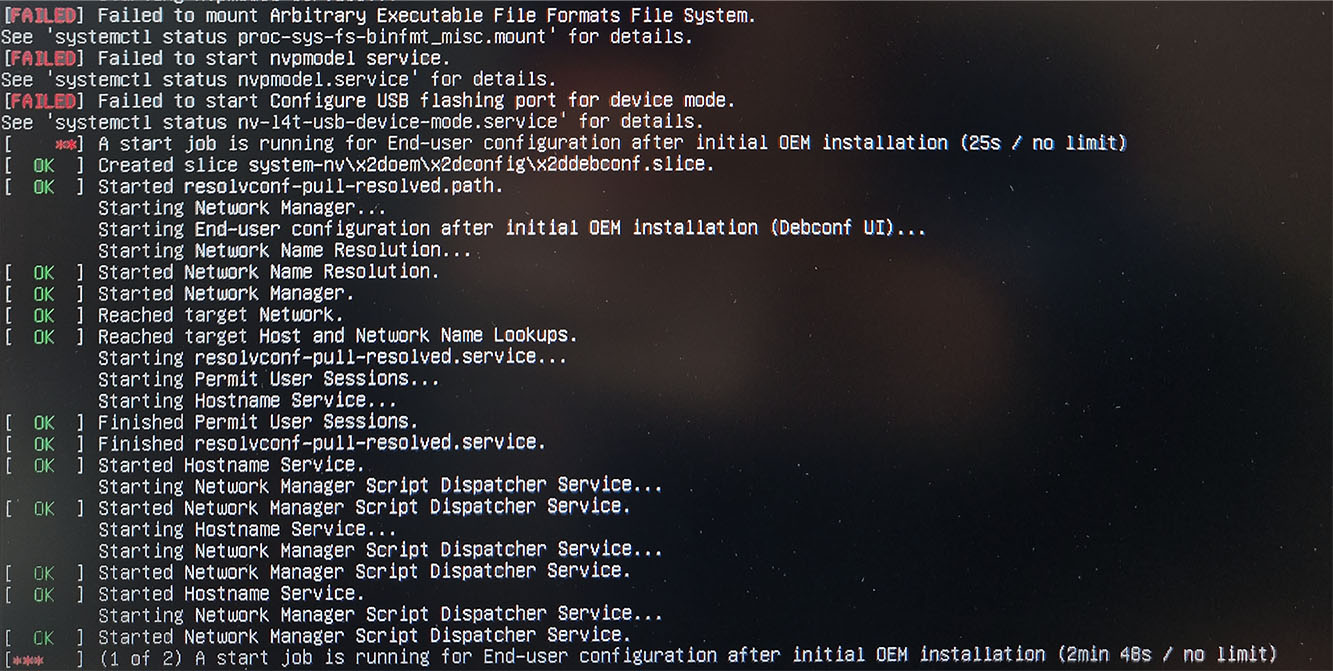
\includegraphics[width=0.8\textwidth]{figures/stuck_in_boot_loop.png}
    \caption{A recurring error when trying to flash the \jx}
    \label{fig:stuck_in_boot_loop}
\end{figure}


\subsection{Improving the workflow}
The second goal was to remove all manual steps from the process.
After flashing the \jx it is normally necessary to connect the \jx to a monitor, keyboard and mouse, and manually create a user.
This is annyoing an time consuming but fortunately there is a script circulating on the \gls{nforum} that can be used to automate this process \cite{waynewwwScriptBypassAccountJun2819}.
Another step that had to be done manually initially was to give the password to different processes to give them sudo persmission.
A simple solution to this was to use the followind code snippet \code{echo <password> | sudo -S <command>}.
Doing this is of course not recommended as it is a security risk, but as a separate laptop was used for this task it was deemed acceptable in this particular case.

The third goal was to make the process faster.
The pipeline was designed to so that it was easy to make checkpoints, so that the entire process did not have to be repeated every time something went wrong.
The compilation it self was also sped up by using all the cores on the computer.

The final goal was to make it easy to include various modifications in the pipeline.
This was acheived by simply adding a new step in the pipeline that would copy the modified files to the right location, or making modifications to the pipeline itself.

After having acheived the four goals above, the script only needed to be started and left alone for a couple of hours before one could \gls{ssh} into the \jx to check the result.

\subsection{Brute force solution}
After having a working automated process for flashing the \jx it was time to start trying to enable \gls{pps} interrupts.
Goin into detail about all the different attempts that were made is not relevant, but a full list of relevant posts from the \gls{nforum} can be found in the appendix if the reader is interested.





\subsection{Preparation}
To flash the \jx it is necessary to have a host computer running Ubuntu 16.04 or 18.04 or 20.04 or 22.04 \cite{nvidiaSDKManager2019}.
Several attempts were made at using the docker image inside \gls{wsl}, communicating with the \jx using usbipd-win, without any success \cite{martensPortableSensorRig2022} \cite{nvidiaSDKManager2019} \cite{dorsselaerUsbipdwin2023}.


